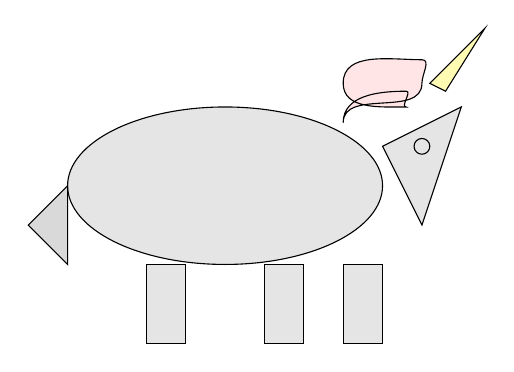
\begin{tikzpicture}
    % Body of the unicorn
    \draw [fill=gray!20] (0,0) ellipse (2 and 1);
    % Legs
    \draw [fill=gray!20] (-1,-1) rectangle (-0.5,-2);
    \draw [fill=gray!20] (0.5,-1) rectangle (1,-2);
    % Tail
    \draw [fill=gray!30] (-2,0) -- (-2.5,-0.5) -- (-2,-1) -- cycle;
    % Head
    \draw [fill=gray!20] (2,0.5) -- (3,1) -- (2.5,-0.5) -- cycle;
    % Eye
    \draw (2.5,0.5) circle (0.1);
    % Horn
    \draw [fill=yellow!30] (2.8,1.2) -- (3.3,2) -- (2.6,1.3) -- cycle;
    % Mane
    \draw[fill=pink!40] (1.5,0.8) to [out=90,in=180] (2.3,1.2) to [out=0,in=180] (2.3,1) to [out=180,in=270] (1.5,1.3) to [out=90,in=180] (2.5,1.6) to [out=0,in=90] (2.5,1.3) to [out=270,in=90] (1.5,0.8);
    % Front leg
    \draw [fill=gray!20] (1.5,-1) rectangle (2,-2);
\end{tikzpicture}